\documentclass{ximera}

\newcommand{\RR}{\mathbb R}
\renewcommand{\d}{\,d}
\newcommand{\dd}[2][]{\frac{d #1}{d #2}}
\renewcommand{\l}{\ell}
\newcommand{\ddx}{\frac{d}{dx}}
\newcommand{\dfn}{\textbf}
\newcommand{\eval}[1]{\bigg[ #1 \bigg]}


\author{Jim Talamo}
\license{Creative Commons 3.0 By-bC}


\outcome{}


\begin{document}
\begin{exercise}
Suppose that $\{a_n\}_{n=1}$ is a sequence and define its sequence of partial sums $\{s_n\}_{n=1}$ by the usual rule $s_n = \sum_{k=1}^n a_k$.  Suppose it is known that:

\[
s_n = \frac{2^n+n^2+1}{3^n}
\]

Then, what is $a_1+a_2$?

\[
a_1+a_2= \answer{1}
\]
\begin{hint}
By definition, $a_1+a_2 = s_2$, so plug $n=2$ into the given formula for $s_n$ to find $a_1+a_2$.
\end{hint}
\begin{exercise}
\[
\lim_{n \to \infty} s_n = \answer{0}
\]
\begin{hint}
Use the Growth Rates Result.
\end{hint}
\begin{exercise}
Since $\lim_{n \to \infty} s_n$ exists, then $\sum_{k=1}^{\infty} a_k$:


\begin{multipleChoice}
\choice[correct]{converges.}
\choice{diverges.}
\end{multipleChoice}

Since the limit $\lim_{n \to \infty} s_n$ is $0$, then $\sum_{k=1}^{\infty} a_k$:
\begin{multipleChoice}
\choice[correct]{converges to 0.}
\choice{converges, but more information is needed to determine its value.}
\end{multipleChoice}

\begin{exercise}
Determine $\sum_{k=3}^{\infty} a_k$.

\[
\sum_{k=3}^{\infty} a_k = \answer{-1}
\]

\begin{hint}
Note that the lower index is different from before.  We have an earlier result that allows us to compute an infinite sum, so in some sense, the heavy lifting has been done.  Indeed, write out the sum we found earlier.
\begin{image}
  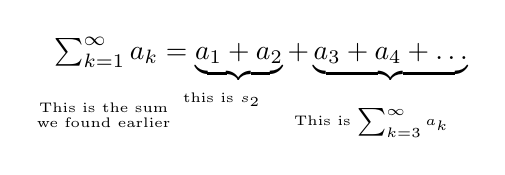
\begin{tikzpicture}
        \node at (0,0) {
          $\sum_{k=1}^{\infty} a_k= \underbrace{a_1+a_2} + \underbrace{a_3+a_4+\ldots}$
        };
        \node at (-.5,-.5) {\tiny{this is $s_2$}};
        \node at (-2,-.6) {\tiny{This is the sum }};
         \node at (-2,-.8) {\tiny{we found earlier}};
        \node at (1.4,-.8) {\tiny{This is $\sum_{k=3}^{\infty} a_k$}};
      \end{tikzpicture}
  \end{image}
\end{hint}

Thus:

\begin{align*}
\sum_{k=1}^{\infty} a_k &= s_2 + \sum_{k=3}^{\infty} a_k \\
\answer{1} &= \answer{2} + \sum_{k=3}^{\infty} a_k
\end{align*}

\begin{exercise}
The series $\sum_{k=1}^{\infty} s_k$: 

\begin{multipleChoice}
\choice[correct]{converges.}
\choice{diverges.}
\end{multipleChoice}

\begin{hint}
Write out the sum you are trying to analyze.

\[
\sum_{k=1}^{\infty} s_k = \sum_{k=1}^{\infty} \answer{\frac{2^k+k^2+1}{3^k}}
\]
This series can be analyzed using either Ratio, Root, or Limit Comparison Test.

\end{hint}
\end{exercise}
\end{exercise}
\end{exercise}
\end{exercise}
\end{exercise}


\end{document}
